%球坐标系

\pentry{位矢\upref{Disp},矢量的叉乘\upref{Cross}}

\subsection{球坐标}

三维直角坐标系中的一点 $P$ 的位置可以用 $(r,\theta ,\phi )$ 这3个有序实数来表示,称为该点的\textbf{球坐标}(\autoref{Sph_fig1}).其中 $r$ 表示该点到原点的距离 $(r \ge 0)$, 即位矢\upref{Disp}的\textbf{模长}; $\theta$ 表示该点的位矢与 $z$ 轴的夹角 $(\theta  \in [0,\pi])$, 即\textbf{极角}; $\phi$ 表示该点的位矢在 $x - y$ 平面上的投影与 $x$ 轴的夹角 $(\phi  \in [0,2\pi]\text{或}[- \pi,\pi])$, 即\textbf{方位角}.注意有些教材中用 $\theta $ 表示方位角, $\phi $ 表示极角,或者将 $\phi $ 记为 $\varphi $,  $r$ 记为 $\rho $ 等,需要通过上下文判断每个坐标符号的具体含义.

\begin{figure}[ht]
\centering
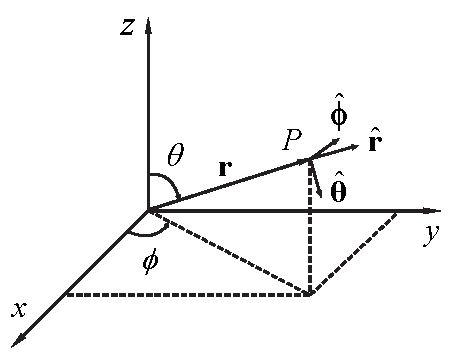
\includegraphics[width=6cm]{./figures/Sph.pdf}
\caption{球坐标系}\label{Sph_fig1}
\end{figure}

\subsection{球坐标系中的单位矢量}
三个球坐标分别有对应的单位矢量 $\uvec r, \uvec\theta, \uvec\phi$ (如图%未完成引用
).定义它们的方向分别指向对应坐标增加的方向,例如 $r$ 增加时,点 $P(r,\theta ,\phi )$ 就向 $\uvec r$ 的方向移动.三个单位矢量两两垂直,形成一组正交归一基底,任意三维矢量都可以表示成它们的线性组合.即
\begin{equation}
\vec v = (\vec v \vdot \uvec r)\,\uvec r + (\vec v \vdot \uvec \theta)\,\uvec \theta  + (\vec v \vdot \uvec \phi)\,\uvec \phi  = v_r \,\uvec r + v_\theta \,\uvec \theta  + v_\phi \,\uvec \phi 
\end{equation}
与直角坐标系不同的是,按照定义,球坐标的三个单位矢量是关于 $\theta$ 和 $\phi$的函数.即
$\uvec r(\theta ,\phi )$,  $\uvec \theta (\theta ,\phi )$,  $\uvec \phi (\phi )$. 
例如 $P$ 的球坐标为 $(1, \pi/2, 0)$, 直角坐标为 $(1, 0, 0)$ 时,
$\uvec r = \uvec x$, $\uvec \theta  =  - \uvec z$, $\uvec \phi  = \uvec y$. 
但是球坐标为 $(1, \pi/2, \pi/2)$, 直角坐标为 $(0, 1, 0)$ 时, $\uvec r = \uvec y$, $\uvec \theta  =  - \uvec z$, $\uvec \phi  =  - \uvec x$. 
一般地,对于球坐标为 $(r, \theta , \phi )$ 的点 $\uvec r, \uvec \theta, \uvec \phi$  与 $\uvec x, \uvec y, \uvec z$ 的关系见球坐标与直角坐标的转换\upref{SphCar}.另外注意改变 $r$ 时 $\uvec r, \uvec \theta, \uvec \phi$ 都保持不变,且 $\uvec \phi (\phi )$ 仅由坐标 $\phi $ 决定.

三个坐标按照 $(r, \theta , \phi )$ 排序,是为了使对应的单位矢量满足 $\uvec r \cross \uvec \theta  = \uvec \phi $ (类比直角坐标系的三个单位矢量必须满足 $\uvec x \cross \uvec y = \uvec z$, 见矢量的叉乘\upref{Cross}). 这也是所有\textbf{正交曲线坐标系}%未完成:词条
 的要求.
 
\subsection{球坐标系中矢量的两种表示方法}
球坐标系中,矢量可以用球坐标 $(r, \theta, \phi)$ 表示,即矢量以原点为起点,以终点的球坐标表示该矢量.

更常见的方法,是将矢量投影到 3 个单位矢量上( 当然,要说明是关于哪个点的单位矢量), 用单位矢量的线性组合来表示.在矢量分析中,这种方法常用于表示\textbf{矢量场}.%未完成:词条

例如任意一点 $P(r, \theta, \phi)$ 的位矢\upref{Disp}都可以表示为 $r\,\uvec r$. 又如原点处电荷 $q$ 产生的电场为 $\vec E = k q \,\uvec r/r^2$. 又如一个绕 $z$ 轴逆时针旋转( 角速度 $\omega $) 的圆柱,在 $P$ 点的线速度为
\begin{equation}
\vec v = \omega r\sin \theta \,\uvec \phi 
\end{equation}









